\section{Research Plan}

{This dissertation proposes an alternative model for urban-decision making. This model embodies a systematic, scalable, evidence-based and data-driven approach, alongside a comprehensive, long-term, and community driven planning. This \textit{New Urban Process}, is manifested in the design, development and deployment of CityScope. CityScope is a human-centered, urban modeling, simulation and decision-making platform, that merges urban technology with social discourse. This section reports on a series of lab experiments and real-world deployments of the CityScope platform, as well as on-going and future CityScope projects.}


\begin{figure}[t]
\begin{center}
    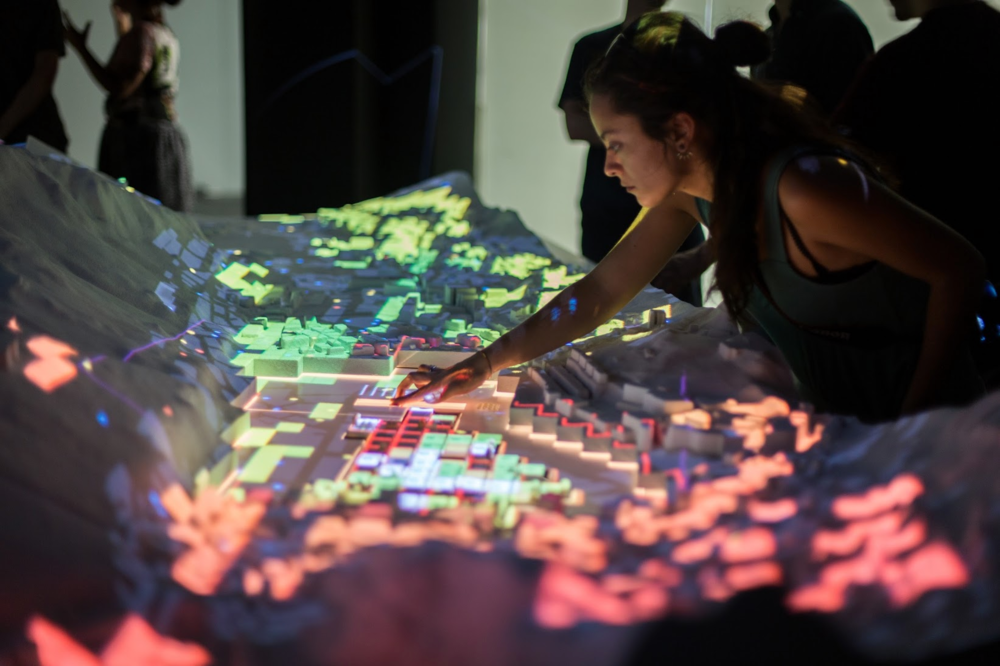
\includegraphics[width=\textwidth]{figures/csl_andorra.png}
\end{center}
   \caption{CityScope Andorra at the City Science Lab in Caldea, Andorra la Vella. Built in 2016, this platform was one of the first to serve as an interactive, real-time tool for urban decision making in real world settings. Here, a user interacts with a Tangible User Interface to asses the impacts of different interventions in the city center.}
\label{fig:csl_andorra}
\end{figure}


\subsection{CityScope: Development Themes}

{Since 2013, CityScope is being developed at the MIT City Science Group, as well as by research labs, companies, and individuals around the world. In this section I cluster CityScope milestones into four major categories: \textbf{Insight}: CityScope as urban observatory, expending on advanced methods in urban and spatial analysis, and focusing on high-resolution, geolocated, urban-dynamics data. \textbf{Predictions}: turning insights into forecasts, using methods of urban modelling and simulation, with an emphasis on real-time predictive models. \textbf{Transformations}: building iterative spatial 'what-if' scenarios through playful and exploratory process. Developing multiple urban-HCI methodologies to engage diverse parties in the urban process. \textbf{Consensus}: Using CityScope to construct multi-stakeholder decision-making, consensus and policy recommendations. Explores Socio-technical systems to facilitate collaborative and distributed urban decision-making.}



\begin{figure}
\begin{center}
    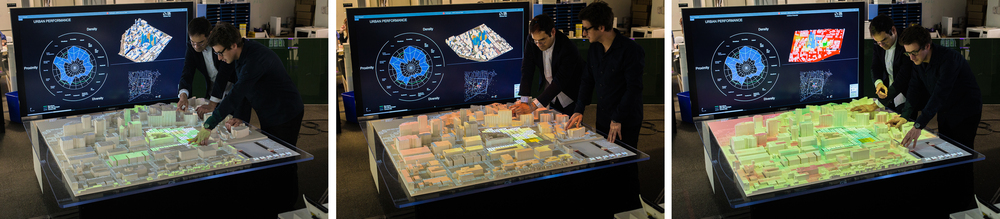
\includegraphics[width=\textwidth]{figures/volpe_all.jpg}
\end{center}
   \caption{CityScope Volpe. This interface explores the development efforts around the MIT campus - DOT Volpe facility. As users interact with the TUI, different matrices update in real-time, to augment multi-party decision-making process. }
\label{fig:volpe_all}
\end{figure}

%%%%%%%%%%%%%%%%%%%%%%%%%%%%%%%%%%%%%%%%%%% 
%%%%%%%%%%%%%%%%%%%%%%%%%%%%%%%%%%%%%%%%%%% 
%%%%%%%%%%%%%%%%%%%%%%%%%%%%%%%%%%%%%%%%%%% 

\subsection{Insight: Observing the City's Current State}

{Urban insights help understand the current state of the city, and can highlight areas in need for change. As highly complex systems of systems \cite{Batty2009}, it is often challenging to focus the planning process on the right urban questions. Narrowing the spectrum of urban observations is a step towards a productive discourse between stakeholders and decision makers. Methodical data collection and representation can also set the stage for more accurate scenarios testing. Early CityScope instances focused on augmenting accessible and concise urban data onto physical 3D platforms, in an effort to facilitate conversations on the city's current performance and plausible interventions. The \textbf{Urban Data Observatory} (2013-2016), displayed various pre-computed urban insights of the MIT and Kendall Square area, such as urban form, physical systems, solar emission, or wind regime.}

{In later CityScope projects, early data exploration and visualization is used to inform the research question and establish KPIs for urban interventions. In \textbf{CityScope Andorra} (2016), observations from Call Data Records and Radio Network Controller data were used to interpret discrete mobility trajectories. Insights gathered from this data could suggest how people move, by which modes of transportation, their daily routines, congregation spots, and the points of interest that attract them. These insights helped create interactive CityScope platforms that can support urban-planning, traffic and energy optimisation, tourism management, as well as COVID-19 mobility policies.}

\begin{figure}
\begin{center}
    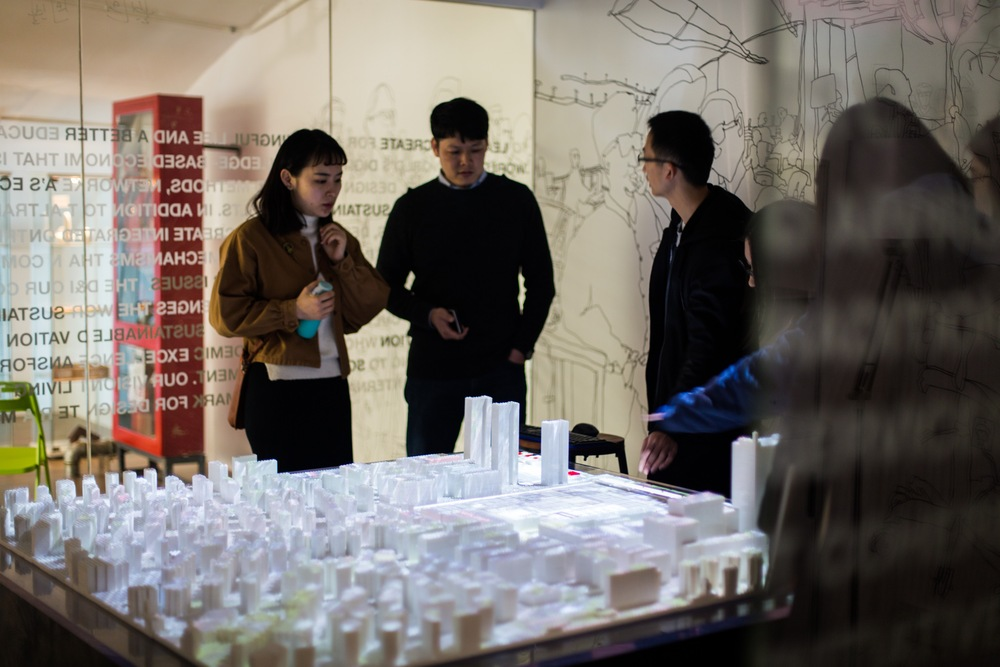
\includegraphics[width=\textwidth]{figures/CSL_tongji.jpg}
\end{center}
   \caption{CityScope LivingLine in Tongji University, Shanghai. Insights with no data: The lack of spatial and behavioral data in this site was compensated by hands-on data aggregation conducted by troves of students.}
\label{fig:CSL_tongji}
\end{figure}

{In places where Location Base Service data is scarce or unavailable, more traditional approach to street observation and data collection can be used. In \textbf{CityScope LivingLine} (2017) in Shanghai, street surveys and physical counts were performed to evaluate small-scale human mobility within a busy shopping area. Similar methodology was  used for the CityScope project in \textbf{Aalto University Campus} in Espoo, Helsinki (2017), where large group of students gathered usage patterns of the campus facilities. Although these methods of data collection are limited, fine-grained recollections of human behavior can go beyond the static representation of spaces, functions and urban systems, and shed light on discrete aspects of urban performance.}

{This thesis will include results from several \textit{insight} related projects, including: Hi-res clustering and analysis of streets vibrancy in Boston; and investigation into the relationship between mobility and COVID-19 spread in Andorra}


\subsection{Transformation}

{The role of CityScope's insights is to focus the discussion on specific urban challenges, and establish clear KPIs to evaluate future interventions. The third step in \textit{a new urban process} is transformation, in which iterative exploration of interventions and policies is performed. In CityScope, testing transformation alternatives is possible through a slew of urban-HCI methodologies and interfaces. Unlike traditional planning and design practices, CityScope is built for dynamic scenario exploration, in which evaluation is conducted synchronously. To allow for fast iterations and real-time feedback, transformation capability is developed via two parallel streams: (i) The creation of iterative user interfaces, such as Tangible User Interfaces, AR, VR, MR, and web-based UIs. (ii) real-time models, simulations, and KPI results which can provide feedback during design sessions.}

\begin{figure}[t]
\begin{center}
    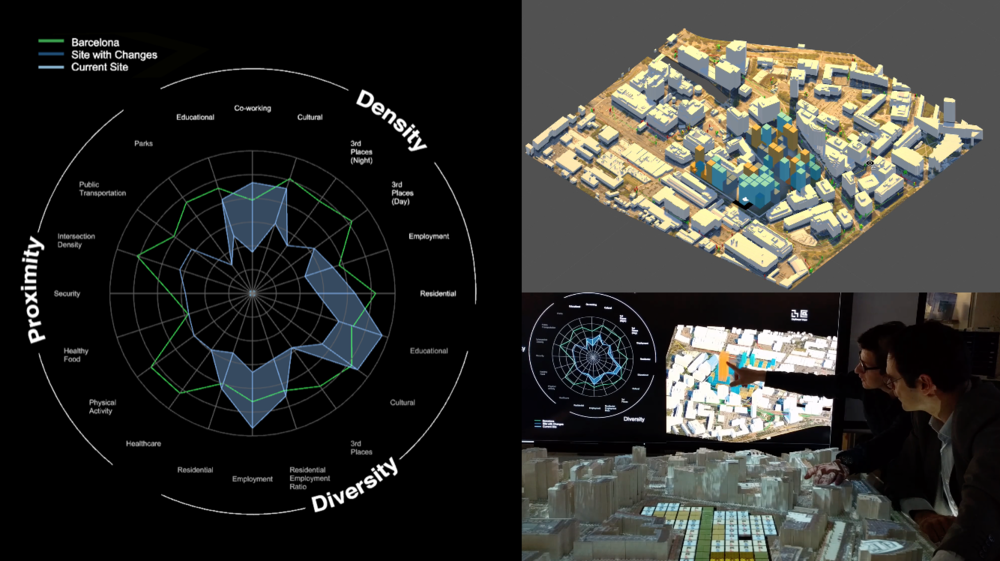
\includegraphics[width=0.8\textwidth]{figures/volpe_ui.png}
\end{center}
   \caption{Urban transformation. Left: a set of KPIs and urban indicators are evaluated with each design iteration. Upper-right: The users interactions are translated to three-dimensional zoning envelops, which represent the maximal intervention framework, rather than actual building volumes. Lower-right: Users are presented with both outputs as a mean to direct their design collaboration process.}
\label{fig:volpe_ui}
\end{figure}


{Different HCI methods were developed in order to digitally capture virtual and physical objects and translate users' interaction into urban transformation. In \textbf{CityScope Playground} (2014-2015), and in the vast majority of CityScope TUIs, a scanning of tagged LEGO bricks allowed near real-time physical-digital interaction. \textbf{CityScopeAR} (2015-2017) added Augmented, Mixed, and Virtual Reality environments that extend CityScope tangible interface. Deployed in the context of \textbf{Boston BRT}, \textbf{Andorra}, and \textbf{Volpe} CityScope projects, this system allowed to enlarge the user-base of participants and curate specific insights to each user. A unified system for obtaining user-interaction from AR devices, LEGO and robotic TUI, and web interfaces was introduced in \textbf{CityScopeJS} (2019).}


{\textit{Transformation} is also the phase in which real-world constraints, such as spatial and legal boundaries are introduced. In \textbf{CityScope Playground}, (2014-2015) an urban simulator design to evaluate building-code and zoning, users explored how existing zoning laws might impact future developments, and suggest zoning amendments. Later transformation projects, such as \textbf{Volpe} (2016-2017), \textbf{Andorra}, (Andorra La Vella 2016-2017), \textbf{Grasbrook} (Hamburg, 2018), and \textbf{Corktown} (Detroit, 2020) included additional site analyses, such as accessibility, spatial diversity of land-use and functions, and various mobility aspects.}

{This thesis will include results from several \textit{transformation} projects, including: the development of a web-based, platform agnostic interaction system for Cityscope; The development of a data standard across CityScope projects; the integration of different TUIs into the platform, such CV based system, actuated interface, as well as touch and web UI.}

%%%%%%%%%%%%%%%%%%%%%%%%%%%%%%%%%%%%%%%%%%% 
%%%%%%%%%%%%%%%%%%%%%%%%%%%%%%%%%%%%%%%%%%% 
%%%%%%%%%%%%%%%%%%%%%%%%%%%%%%%%%%%%%%%%%%% 

\subsection{Prediction: Urban `What-if' Scenarios}

{The ability to predict the future of urban environments is a critical aspect in urban planning, urban design, and architecture. Unlike other industries, urban interventions rarely permit processes of trial-and-error and A/B testing, thus requiring high degree of confidence and well established predictive models \cite{doi:10.1080/14649357.2015.1127994}. As depicted in figure \ref{fig:axis}, urban predictions could be generally described using two vectors: (I) the prediction time-frame, and (II) the social to physical spectrum.}

\begin{figure}[t]
\begin{center}
    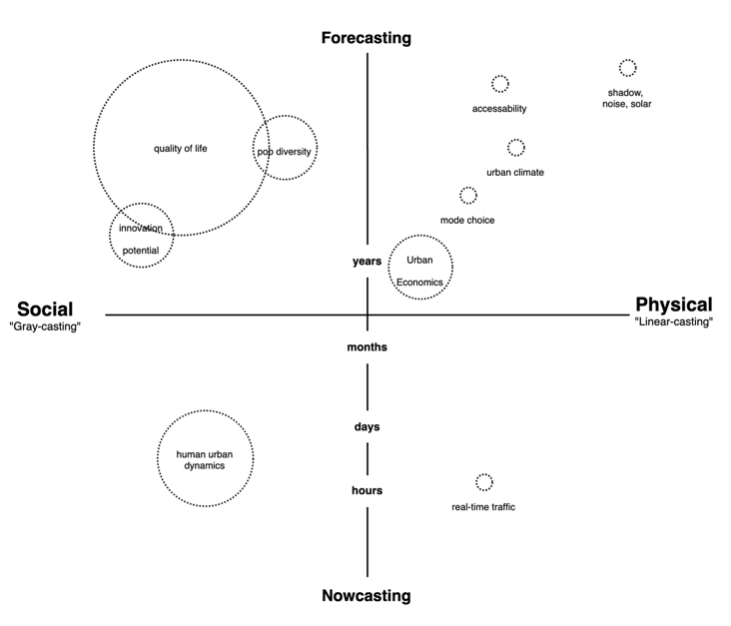
\includegraphics[width=0.7\textwidth]{figures/prediction_axes.png}
\end{center}
   \caption{The landscape of urban prediction. The horizontal axis represents the degree of `concreteness' of each prediction (social <-> physical). The vertical axis depicts the longevity of the prediction (now <-> far future).}
\label{fig:axis}
\end{figure}

{As an example, predicting the shadow effect of a new building on the streetscape is linearly correlated to its bulk and shape. Evidently, as long as the world spins around the sun, the results of shadow modelling should be consistent, and the model describing this phenomena could be reused indefinitely. On the other end, a predictive model of potential human interaction in a public plaza, would share much less consistency across time and space. This model would heavily rely on social and cultural aspects, as well as physical attributes of the urban realm (such as the plaza's shape, or its proximity to certain amenities). This class of predictions, which focuses on human-urban dynamics, is dramatically harder to construct, validate and reuse, but can carry greater impact on decision-making.}

{Today, many commercial and research tools already offer high-accuracy and efficiency in physical urban prediction. This dissertation focuses on the other class of predictions, at the intersection of human behavior and the built environment. The \textbf{Reversed Urbanism} (2017-2018) project attempted to model and predict the propensity of certain human behavioral patterns in public spaces
 (see figure \ref{fig:revurb}). These models meshed geo-spatial attributes (such as urban form, POIs, and street network graphs), and socio-behavioral properties, interpreted from high-resolution telecom data. Later CityScope projects, such \textbf{Corktown}, and \textbf{Grasbrook} take similar approach when meshing geospatial data with hi-res location data to conduct mobility predictions.}



\begin{figure}[t]
\begin{center}
    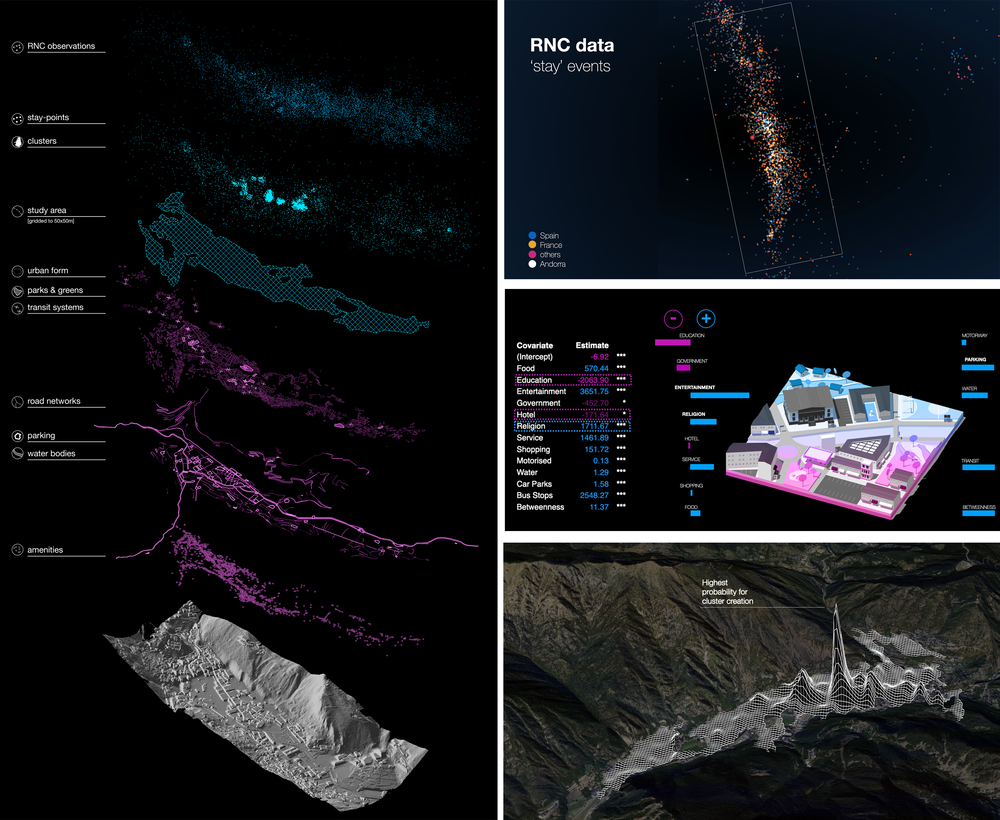
\includegraphics[width=0.9\textwidth]{figures/revurb.png}
\end{center}
   \caption{The Reversed Urbanism project. Left: various layers of spatial and behavioral data are meshed to create a spatio-temporal understanding of the cityscape. Upper-right: high-resolution geo-located telecom data is processed as `stay events', in which users stayed above a certain spatio-temporal threshold. Mid-right: The degree of correlation between clusters of stay-events and different spatial features are modelled for each cell on an arbitrary grid. Lower-right: the model can then predict the propensity of each cell to attract these clustered behaviors.}
   
\label{fig:revurb}
\end{figure}

{When geo-located data are scarce or unavailable, other techniques could be used to simulate urban dynamics. In \textbf{CityScope MoCho} (2019), mobility mode-choice patterns for the Boston metro area were simulated using synthetic population. Static data, such as census and National Household Travel Survey (NHTS) were used to construct simulated profiles of daily commuters. By interpreting plausible trips from socio-demographic data, the model could predict how fairly small scale changes to land-use (performed via CityScope TUI) can affect large scale mobility behaviors.}

{Simulated populations can also help to understand emergence and agglomeration patterns, and can inform design decisions. In CityScope \textbf{Volpe}, \textbf{Andorra}, \textbf{Grasbrook} and \textbf{Champs-Élysées} (2016-2020) Agent Based Models (ABM) are used to simulate travel patterns and mobility choices as a result of land-use and urban-design transformations. A similar approach was used in the \textbf{Hamburg Port-City Model}, in which an ABM was used to predicate changes to tourist activity in train-stations and the harbor port. In these cases, when mobility data was insufficient, virtual populations were formed to model and predict the impact of urban intervention. }


\begin{figure}[t]
\begin{center}
    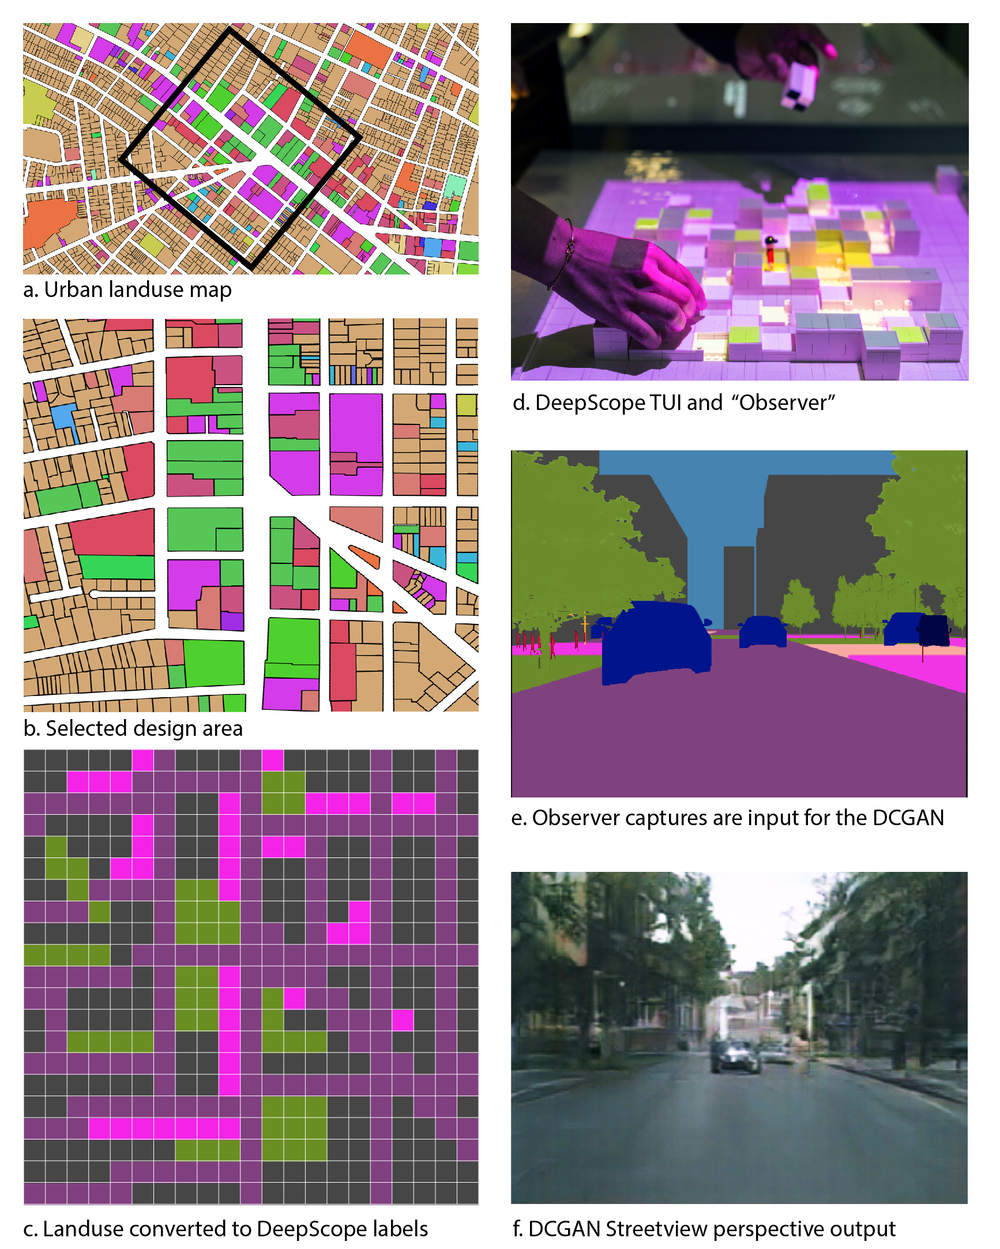
\includegraphics[width=0.6\textwidth]{figures/landuse.jpg}
\end{center}
   \caption{DeepScope module: (a,b) designating an urban intervention site (c) translating the site's land-use/zoning bounds and (d) user-interaction into (e) procedural 3D environment and (e) passing it to DCGAN model for generation of a street-view visualization}
\label{fig:landuse}
\end{figure}
{A different aspect of CityScope predictions involves the usage of data-driven models to forecast changes in urban environments. These models can expedite traditionally complex and slow urban analytics, as well as generate a slew of possible iterations for each design question. The \textbf{DeepScope} (2019) project uses Generative Adversarial Networks to predict and render streetscapes of areas under development in real-time. The goal of this CityScope module is to expedite traditional urban design processes, and offer real-time visualization during early massing exercises. Similar models use Convolutional Neural Networks to expedite CityScope predictive capabilities (such as innovation potential, urban mobility, economic performance, sustainable buildings, or community benefits), and replace them with pre-trained, real-time predictions.}

{This thesis will include results from several \textit{prediction} projects, including: the development and testing of real-time modelling framework for CityScope; publication of real-time mobility model for Detroit; and the usage of pre-trained machine learning models to reduce computation overhead in Hamburg.}

\begin{figure}[t]
\begin{center}
    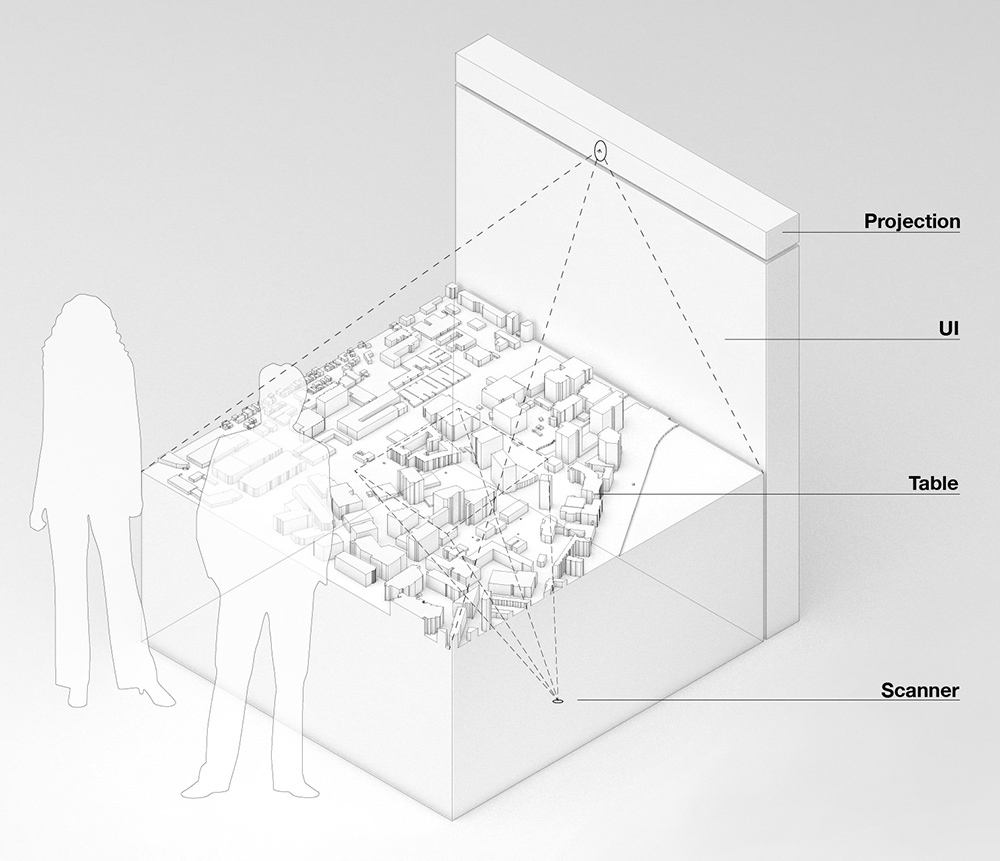
\includegraphics[width=0.6\textwidth]{figures/CityScope TUI.jpg}
\end{center}
   \caption{Common architecture of CityScope TUI: Multiple users can simultaneously interact and discuss urban design iterations. The table-top is used as both the design space and a schematic urban top-view. The vertical monitor visualizes additional insights and predictions. Sensors/cameras scan the scene for real-time interaction.}
\label{fig:CityScopeTUI}
\end{figure}

%%%%%%%%%%%%%%%%%%%%%%%%%%%%%%%%%%%%%%%%%%% 
%%%%%%%%%%%%%%%%%%%%%%%%%%%%%%%%%%%%%%%%%%% 
%%%%%%%%%%%%%%%%%%%%%%%%%%%%%%%%%%%%%%%%%%% 

\subsection{Consensus}

{The last phase, and probably the most impactful in \textit{the New Urban Process} is the establishment of consensus between diverse stakeholders. Too often, planning processes are invested in the envisioning of urban futures through data, simulation, and design iterations, but fail to include stakeholders and the public in these processes.} 

{In the core of CityScope is the notion that planning efforts must be conducted in a shared, collaborative, and engaged way. This approach promoted the design of the platform, the development of its computational models and modules, as well as the creation of community engagement processes that revolve around these technologies. \textbf{CityScope Boston BRT} (2014-2015), a community engagement process for the planning on Bus Rapid Transit routes, brought together a range of urban HCI technologies with public participation. This process aimed to go beyond common community engagement sessions which range between information-sharing to venting, and instead was designed around co-creation and citizen-driven planning. In this case, CityScope was not only a planning and urban transformation tool, but also as a medium supporting debate and evidence-based discourse by different parties.}


\begin{figure}[!tbp]
  \centering
  \begin{minipage}[b]{0.48\textwidth}
    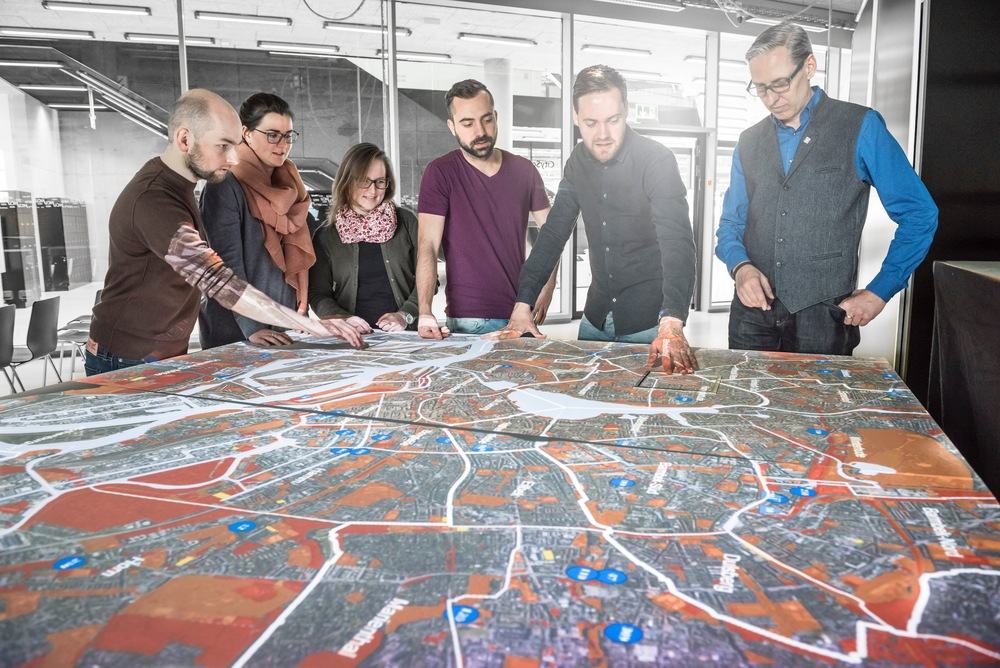
\includegraphics[width=\textwidth]{figures/finidingplaces1.jpg}
  \end{minipage}
  \hfill
  \begin{minipage}[b]{0.48\textwidth}
   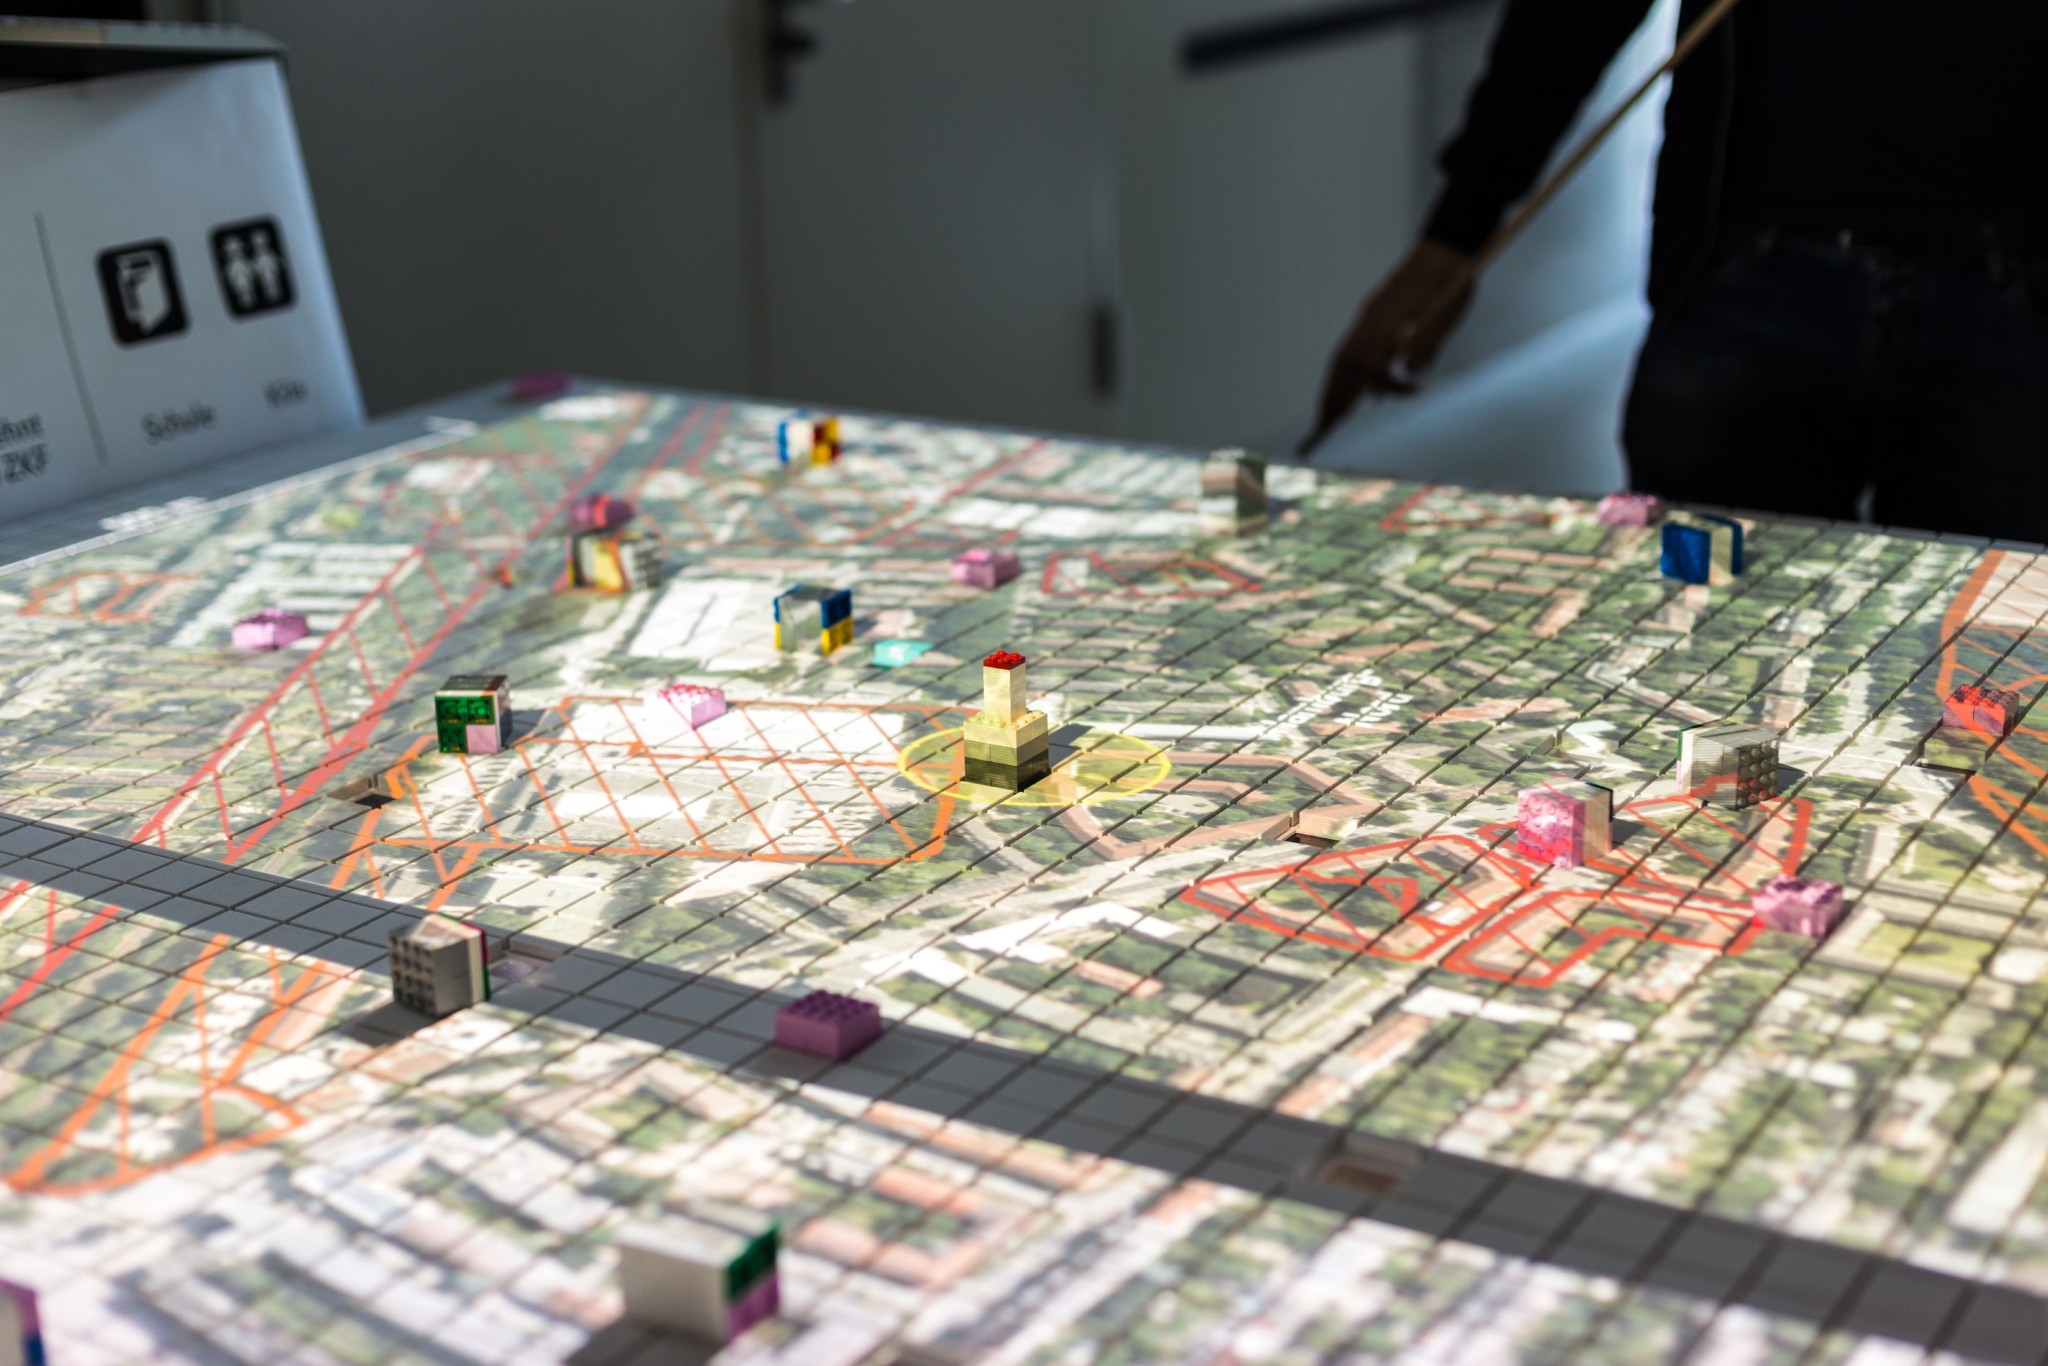
\includegraphics[width=\textwidth]{figures/finidingplaces0.jpg}
  \end{minipage}
    \hfill
   \caption{CityScope FindingPlaces TUI: Users could add or test housing volumes in different configurations. The system would react by prompting on potential risks or issues, such as land contamination, proximity to power-lines, etc.  }
\end{figure}


{The lessons learned about community engagement and public participation using CityScope, were put into extreme test in the \textbf{FindingPlaces} (2015-2016) project. In late '15, the City of Hamburg faced an escalating crisis amidst a massive wave of refugees arriving from war zones in the Middle-East. Here, CityScope FindingPlaces was central in a region-wide effort to construct a public agreement on where and how to host these refugees. CityScope FindingPlaces introduced multiple improvements to current platforms, including agile geographic system, based on real-time GIS, distributed system for interaction instancing, large-scale TUI, as well as a dedicated front-end and back-end architecture. This project also involved an in depth preparation including dedicated participants outreach, orchestrated community sessions, and structured documentation and reporting mechanisms. FindingPlaces proven the ability of CityScope to become pivotal platform for consensus-building amongst diverse stakeholders, that can convert even heated urban debated into tangible solutions.}